\documentclass{article}
\usepackage{tikz-qtree}
\begin{document}
\tikzset{every tree node/.style={minimum width=2em,draw,circle},
blank/.style={draw=none},
edge from parent/.style={draw,edge from parent path={(\tikzparentnode)--(\tikzchildnode)}},
level distance=1.5cm}
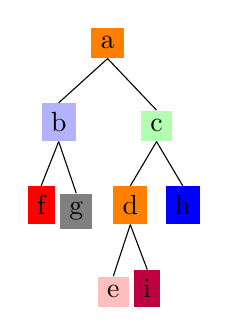
\begin{tikzpicture}

\Tree
[. \node[fill=orange]{a};
[. \node[fill=blue!30]{b};
\edge[]; \node[fill=red]{f};
\edge[]; \node[fill=gray]{g};
]
[. \node[fill=green!30]{c};
\edge[]; [. \node[fill=orange]{d};
\edge[]; \node[fill=pink]{e};
\edge[]; \node[fill=purple]{i};
]
\edge[]; \node[fill=blue]{h};
]
]

\end{tikzpicture}
\end{document}
